\documentclass[11pt, oneside]{article} 
\usepackage{geometry}
\geometry{letterpaper} 
\usepackage{graphicx}
	
\usepackage{amssymb}
\usepackage{amsmath}
\usepackage{parskip}
\usepackage{color}
\usepackage{hyperref}

\graphicspath{{/Users/telliott/Github/calculus_book/png/}}
% \begin{center} 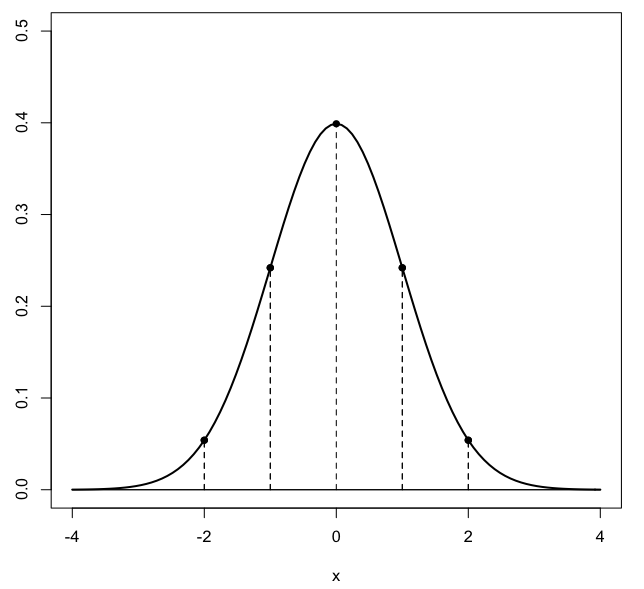
\includegraphics [scale=0.4] {gauss3.png} \end{center}

\title{Pythagorean Algebraic Proofs}
\date{}

\begin{document}
\maketitle
\Large

\label{sec:pythagoras_algebraic}

\subsection*{algebraic proofs}

The following proofs are algebraic ones.  Not so pretty, but fast.  

Arrange 4 identical right triangles as shown in the figure below.  The four triangles plus a small central square form a larger quadrilateral which is also a square.

\begin{center} 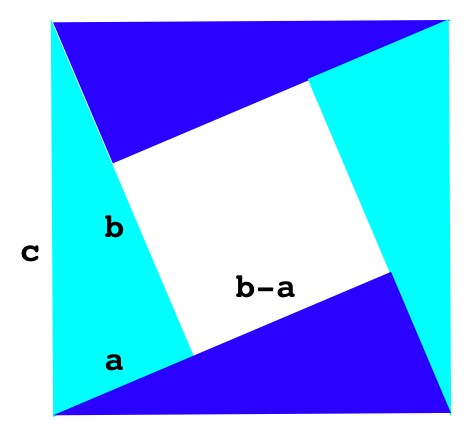
\includegraphics [scale=0.4] {pythagoras5.png} \end{center}

The angles at the corners of the quadrilateral, at the points flanking the hypotenuse $c$, are right angles, because they are formed by addition of two complementary angles of congruent right triangles.  Since the quadrilateral has four internal right angles and equal length sides, it is a square.

Now just calculate the area of the parts.  We have four identical right triangles with sides $a$ and $b$, plus the central square with sides $b-a$.  The area is 
\[ A = 4 \cdot \frac{1}{2}ab + (b - a)^2 \]
\[ = b^2 + a^2 \]

But the area is also the square of side $c$.  

$\square$

We have used various properties proved earlier, e.g. that the sum of the angles of any triangle is $180$ degrees.

Here is a very similar proof:

\begin{center} 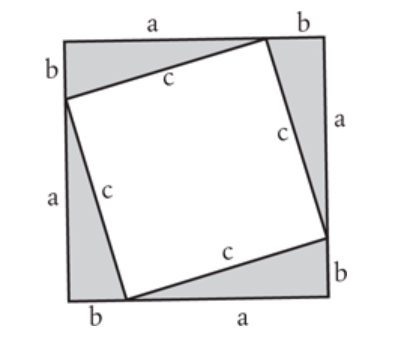
\includegraphics [scale=0.5] {pythagoras6.png} \end{center}

In this figure, the right triangles are aligned so that the big square has sides which combine the lengths $a + b$ and have area $(a + b)^2$.  But we can also calculate the area as the sum of its components, namely, central tilted square plus the four triangles:

\[ (a + b)^2 = c^2 + 4 \cdot \frac{ab}{2} \]
\[ a^2 + b^2 + 2ab =  c^2 + 2ab \]
\[ a^2 + b^2 = c^2 \]

$\square$

For the third algebraic proof, divide a right triangle into two smaller ones by dropping an altitude, which meets the base at a right angle.
\begin{center} 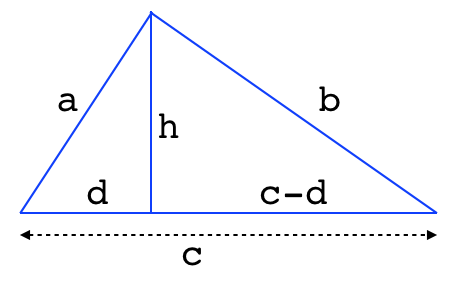
\includegraphics [scale=0.5] {right_triangle.png} \end{center}

By complementary angles, these three triangles are all similar (e.g., the angle between sides $b$ and $h$ is equal to that between sides $c$ and $a$).  

So we can construct ratios of sides that are equal.  There are three sets, here is one:
\[ \frac{a}{c} = \frac{h}{b} = \frac{d}{a}  \]

We have above a relationship from which to construct $a^2$.
\[ a^2 = cd \]

Another relationship is:
\[ \frac{b}{c} = \frac{c-d}{b} = \frac{h}{a} \]
giving this for $b^2$
\[ b^2 = c(c-d) \]

Simply adding the two together yields:
\[ a^2 + b^2 = cd + c(c-d) = c^2 \]

Which is what we wanted to prove.  $\square$

There are more than 300 proofs of this theorem, including one by a President of the United States, James A. Garfield.  

Here is his proof:
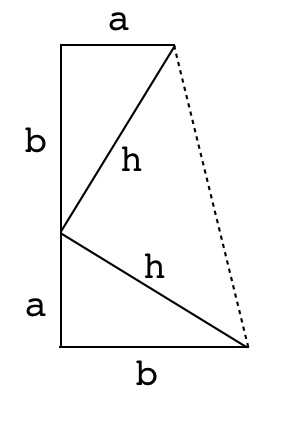
\includegraphics [scale=0.4] {garfield.png}
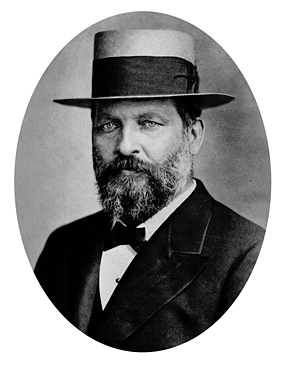
\includegraphics [scale=0.4] {garfield2.png}

Draw a right triangle and a rotated copy as shown.  The area of the quadrilateral is the product of the side $(a + b)$ and the \emph{average} of $a$ and $b$:
\[ A = (a+b) \cdot \frac{1}{2} (a + b) \]
If you don't see this right away, calculate the area as a rectangle plus a triangle (whose side is not shown but drops vertically from the top right corner).
\[ a(a + b) + \frac{1}{2}(b-a)(a+b) \]
with the same result so
\[ A = \frac{1}{2} a^2 + ab + \frac{1}{2} b^2 \]
But it is also the sum of 
\[ \frac{1}{2} ab + \frac{1}{2} ab + \frac{1}{2} h^2 \]
Equate the two and the result follows almost immediately.

$\square$
 
\end{document}